\documentclass{gretsi}
  
  
\usepackage[english,french]{babel}   % "babel.sty" + "french.sty"

% \usepackage{french}                  % "french.sty"
\usepackage{times}			% ajout times le 30 mai 2003
\usepackage{subfig}
\usepackage{graphicx}
\usepackage[justification=centering]{caption}
\usepackage{amsmath}
\usepackage[linesnumbered,ruled]{algorithm2e}
%\usepackage{enumitem}
%% --------------------------------------------------------------
%% FONTS CODING ?
% \usepackage[OT1]{fontenc} % Old fonts
\usepackage[T1]{fontenc}  % New fonts (preferred)
%% ==============================================================

\title{SIFT descriptor to set landmarks on biological images}

\author{\coord{Van Linh}{LE}{1,3},
        \coord{Marie}{BEURTON-AIMAR}{1},
    \coord{Adrien}{KRAHENBUHL}{1},
    \coord{Nicolas}{PARISEY}{2}}

\address{\affil{1}{Laboratoire Bordelais de Recherche en Informatique (LaBRI) \\
         351, cours de la Lib�ration, F-33405 Talence cedex, France}
         \affil{2}{Institute for genetics, the environment and plant protection (IGEPP), INRA 1349  \\
         35653, Le Rheu, France}
         \affil{3}{Faculty of Information Technology, Dalat university  \\
         1 Phu Dong Thien Vuong, Dalat, Lamdong, Vietnam}}

%% If all authors have the same address %%%%%%%%%%%%%%%%%%%%%%%%%%%%%%%%%%%%%%%
%                                                                             %
%   \auteur{\coord{Michel}{Dupont}{},                                         %
%           \coord{Marcel}{Dupond}{},                                         %
%           \coord{Michelle}{Durand}{},                                       %
%           \coord{Marcelle}{Durand}{}}                                       %
%                                                                             %
%   \adress{\affil{}{Laboratoire Traitement des Signaux et des Images \\      %
%     1 rue de la Science, BP 00000, 99999 Nouvelleville Cedex 00, France}}   %
%                                                                             %
%                                                                             %
%%%%%%%%%%%%%%%%%%%%%%%%%%%%%%%%%%%%%%%%%%%%%%%%%%%%%%%%%%%%%%%%%%%%%%%%%%%%%%%

\email{van-linh.le,beurton,adrien.krahenbuhl@labri.fr, nparisey@rennes.inra.fr}


\frenchabstract{L'analyse d'images est une des �tapes majeures du
  traitement d'images num�riques, on l'applique aussi bien en imagerie
m�dicale ou biologique, en vision par ordinateur ... Classiquement,
l'image est tr�s pr�sente en biologie, les differentes techniques
d'acquisition (photosdepuis l'imagerie microscopique
pour �tudier les structures anatomiques jusqu'au scanner, tomographie
ou IRM pour �tudier les tissu}

\englishabstract{Image analysis is a large field of digital image
  processing and it has applied in practice with many application in
  the different majors such as medicine, machine vision, biology,
  ... In the traditional of biology techniques, microscopic techniques
  were applied to study the structure details, but the current
  research requires more accuracy in the area, perimeter, localization
  of the object in the image by using the suitable features. In this
  content of this paper, we will focus on the problem of setting the
  landmarks on biological images which are used in many biological
  studies. The landmarks are indicated by applying a combination of
  SIFT and some techniques. Besides, we also show a difference way to
  use SIFT descriptor with another size of the sample region. The
  efficiency of the method is evaluated on two set of images: left and
  right mandibles of beetle. The complete work is implemented in
  MAELab and freely available as a library.}


\begin{document}
\maketitle

\section{Introduction}
Morphometry analysis is an important field of image analysis in
biology. It is used to characterize the shape variations of the
organisms. From obtained information, the biologists can evaluate the
evolution of an organism or detect differences between several ones. Depending on the requirements of the application, the
output of analysis process can be measures of shape, color ... or
identificaton of pattern or landmark (points of interest) positions. Landmarks are
points along an image outline that store a lot of important
information about the shape of the image. The morphometric landmarks
are precise points defined by the biologists. They are used in many
biological studies and included into the classification tasks. Until
now, the morphometric landmarks are manually identified mainly. The
manual identification is time-consuming and could vary a lot depending on
the operator.


\begin{figure}[h]
\centering
\subfloat[Left mandible]{\label{figrbox2}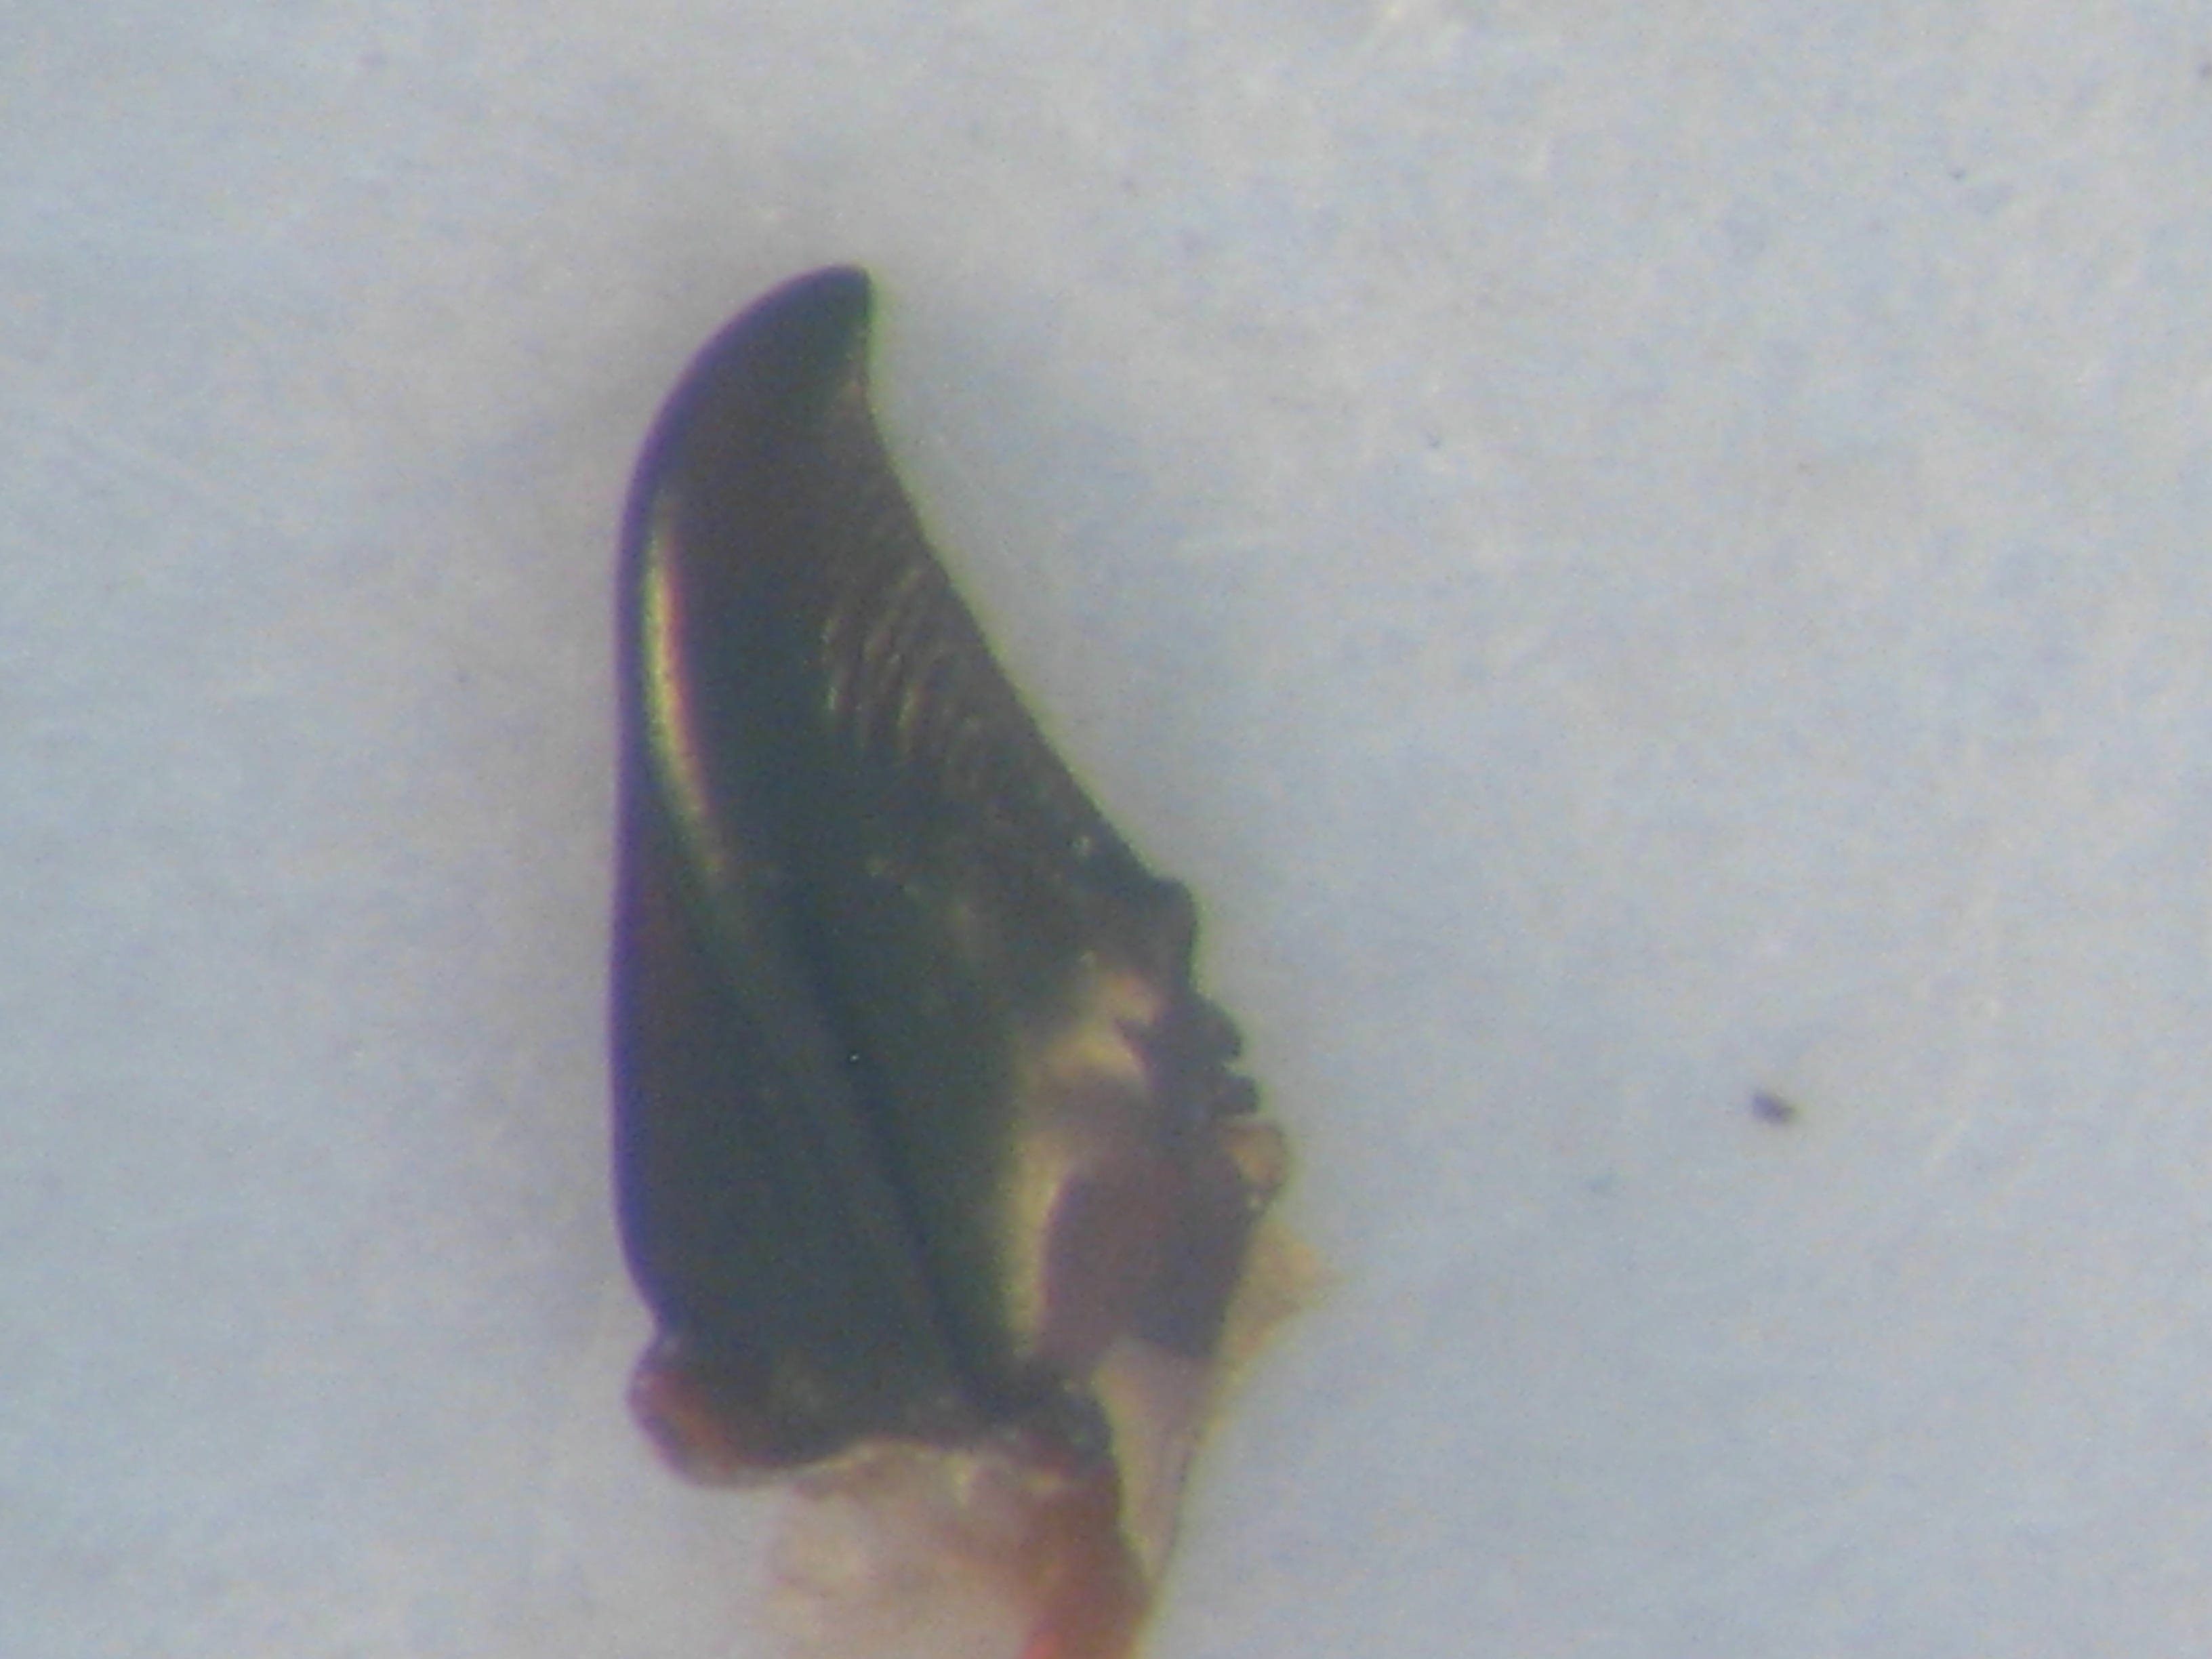
\includegraphics[width=0.22\textwidth]{./images/lm}}~~
\subfloat[Right mandible]{\label{figrbox1}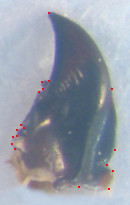
\includegraphics[width=0.22\textwidth]{./images/rm}}
\caption{Example of beetle mandibles from the studied data set.}
\label{fig1}
\end{figure}

In this paper, we focus on the method to automatically determine the
landmarks in 2D biological images (see Fig. 1), specifically beetle
images. The proposed method consists segmentation, registration, and
descriptors comparison techniques. Besides, this method is also shown
as a difference ways to apply the SIFT descriptor for keypoint
detection. The work is evaluated on the dataset of beetles from
Brittany lands with a collection of 293 beetles. For each beetle, a
set of landmarks has been manually located by the biologists. In our
study, we used that dataset as ground truth to evaluate the position
of the automatically estimated landmarks.

\section{Landmark descriptor}
For each beetle, the morphometric landmarks have been manually
identified on mandibles images by the biologists: 16 and 18 landmarks
for each left and right mandible, respectively. The consideration
problem is how to detect automatically the landmarks on the mandible
image to replace the manual ones. In the whole of the process, a
source and a target image are used. The landmarks will be estimated on
the target image by using the manual landmarks of the source
image. Note, the source image is chosen randomly from the set of
images.


In this section, firstly, we have a summary about the general
utilization of SIFT. Then, we will discuss detail about our method
with a difference way of SIFT to estimate the landmarks.

\subsection{SIFT method}
\label{secSIFT}
SIFT method has been proposed by Lowe \cite{lowe1999object,
  lowe2004distinctive}. It is used to extract distinctive invariant
features from the images. Besides, the features from SIFT can use to
match between different views of source and target images such as
rotation, scale, noise. SIFT method includes four stages: (1)
scale-space extrema detection stage, (2) keypoint localization, (3)
orientation assignment, and (4) keypoint descriptor.


In the first stage, a difference of Gaussian (DoG)
\cite{davidson2006molecular}  function is applied to identify the
interest points on all scale and orientation of image. The keypoints
are taken as the maximal and minimal of the result of DoG function at
mutliple scale.

The scale-space extrema detection produces too many kepoint
candidates, some of them are unstable. In the second stage of SIFT,
the key point candidates are localized and refined by suppress the key
points which have the low contrast or are poorly localized along an
edge.

Then, the orientation and gradient magnitude of key points are
calculated by considered the 4-neighborhoods of them.

At the end, the descriptor is computed for each key point based on the
orientation and gradient magnitude. This is the descriptor of a region
$16 \times 16$ pixels around the key point.
\\
By applying the original SIFT into our problem, we have succeeded
indicating the keypoints in the image (see Fig. \ref{fig3}). But we do
not have the result when we try to extract correspondence keypoints
between the source and target image. The problem is carried from the
choosing the best points from the large set of the candidates. This
problem is solved in our method by limit the search space before
applied the SIFT, plus changing the size of the grid to calculate the
SIFT descriptor.

\begin{figure}[htb]
    \centering
    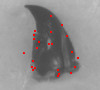
\includegraphics[width=0.3\textwidth]{./images/siftc}
    \caption{SIFT keypoints in a right mandible}
    \label{fig3}
\end{figure}
\subsection{SIFT using into landmark area}
As mentioned in section \ref{secSIFT}, we have tried to use original
of SIFT to detect the landmarks. But the result shows a lot of
candidates for the estimated landmarks. Additional, the position of
the detected points are very far when we compare with the ground truth
ones (manual landmarks), and searching in whole image is very time
consuming. To hope for a better result, we use the SIFT method with
another way, we do not consider all points of the image as
usually. Instead, we limit the searching space and change the region
size around the landmark first.


Firstly, two images are segmented. Then, we register two lists of
contours points. After that, the area (called patch) around each
source landmark is detected then a larger patch is extracted in the
target image at the same position. The SIFT descriptor is calculated
as the original way. But we have reduced two first stages of SIFT and
have changed the size of the sample region as $9 \times 9$ (instead
$16 \times 16$). This size has been obtained after several tests. The
SIFT descriptor for the patch is also an histogram containing the sum
of pixel gradients for each consider direction. The comparison between
two SIFT-descriptors is done by L2-distance with following equation
(Eq. \ref{eql2}):

\begin{equation}
\label{eql2}
	L(D1,D2) = \sum\limits_{i = 0}^{n}\sqrt{(D1_i-D2_i)^2}
\end{equation}
Where:
\begin{itemize}%[nosep,label=\footnotesize$\bullet$]
	\item $n$ is the number of directions
	\item $D1$ and $D2$ are two descriptors of size $n$,
	\item $D1_i$ and $D2_i $ are the $i^{th}$ descriptor values.
\end{itemize}
The way that we apply SIFT into our work is painted in
Fig. \ref{fig4}. To detect the target landmarks, a registration is
computed between the source and target images. Then, the patch $P_m$
of source and $P_s$ of the target are created with the size of $P_m$
is smaller than the size of $P_s$. For each pixel in $P_s$, a
sub-patch $P_s'$ is extracted with the same size of $P_m$. When the
$P_s'$ have a part outside of $P_s$, the pixels do not belong to the
patch will be considered. Then, the distance $L(P_m,P_s')$ is computed
by using Eq. (\ref{eql2}). This work is finished when all the pixel in
patch $P_s$ are considered. The position of estimated landmark
corresponds to the position of the sub-patch $P_s'$ with smallest
distance $L(P_m,P_s')$. Finally, the position of the estimated
landmarks are set in the original position of the target image.

\begin{figure}[htb]
    \centering
    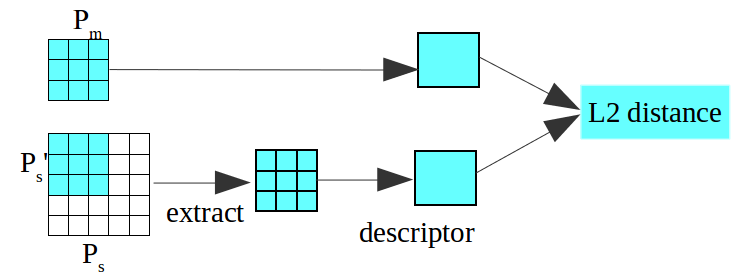
\includegraphics[width=0.48\textwidth]{./images/illustration_SIFT}
    \caption{Steps of SIFT descriptors comparisons between the patch $P_m$ of the source image and the patches $P'_s$ of the target image.}
    \label{fig4}
\end{figure}

By experiments, a patch sample of $9 \times 9$ pixels centered in each
landmark on the source and the size of $36 \times 36$ is kept for the
patch on the target image.

\section{Experiments and results}
The method is tested on two sets (left and right mandible) of
beetles. After verifying the dataset, it remains 290 images of right
mandibles and 286 left mandible images. In all valid images, a set of
manual landmark is indicated by biologists: 18 for each right
mandible, 16 for each left mandible.


As discussed, before applying the SIFT descriptor to estimate the
landmarks on the target image. We have estimated the search space that
contains the landmarks.


Firstly, the segmentation is applied on both of source and the target
image. The Canny algorithm \cite{canny1986computational} was chosen to
finish this step. To use the Canny algorithm, two thresholds value
must be provided ($T_{lower}, T_{upper}$). As mentioned in
\cite{adaptiveCanny}, indicating the threshold values is a difficult
problem. If the threshold values are unsuitable, the contours could be
far with ground truth (fewer contours or more noise). In our case, the
lower threshold value is indicated by analysis the histogram of the
image \cite{leestimating}. The ratio of two threshold values is chosen
as $1 : 3$ to consider a wide range of the values. During Canny
computing, the direction of the gradient of each pixel belonging to
the contours is kept and will be used later. At the end of
segmentation step, a simple algorithm is applied to remove the edge
inside the main contours.


Then, the PCA iteration is computed to register two lists of contours
points from the images \cite{shlens2014tutorial,
  jolliffe2002principal}. The lists of contour points are used  as the
input. The centroid point and principal axis are computed for each
image contours. Two lists of contours points are registered by
computing the translation and rotation parameter values. However in
some case, the result of the segmentation step could exist the noise,
it could affect to the registration step. To improve the registration,
we have built up the PCA by iterating until stabilization
(PCAI). Finally, the SIFT descriptor is finished to determine the
estimated landmark on the target image.


We have run the method on all usable images. The results are given in
difference: estimated landmarks are well positioned on some target
images but not pleasing on others. As raised, the mandible images can
be exist difference sizes because beetles have also difference
sizes. We detected that our method is sensible to this parameter. To
improve the result, we have inserted a pre-process step before the
computing of the SIFT descriptor to estimate the scale between source
and target image. The bounding box of contours in source and target
are defined by checked the coordinate of the contour points. The scale
between two images is the ratio of two bounding boxes.


The Fig. \ref{fig5} shows the final result for a right and a left
mandible with manual and estimated landmarks. The estimated landmarks
are quite near with the manual ones.


\begin{figure}[h]

\centering
\subfloat[Left mandible]{\label{figrbox2}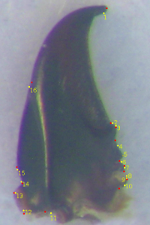
\includegraphics[width=0.22\textwidth]{./images/mg_rs}}~~
\subfloat[Right mandible]{\label{figrbox1}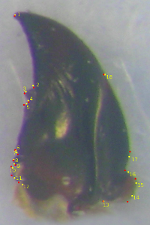
\includegraphics[width=0.22\textwidth]{./images/md_rs}}
\caption{The manual (in red) and estimated (in yellow) landmarks on a mandible.}
\label{fig5}
\end{figure}

The first statistic is done on the mean accuracy of all landmarks on
the target images. The error is computed as the distance between the
manual and corresponding estimated landmark on the target image with
an error accepted from 1\% to 2\% of bounding box's size (when we
consider the scale of the image). According to this way, the result is
shown in Fig. \ref{fig6}; following that, the good score of
well-positioned landmarks equal to \textbf{87.03\%} for the set of
right mandibles and \textbf{78.82\%} for left mandibles.

\begin{figure}[h]
\centering
\subfloat[Set of right mandibles.]{\label{figmdresult}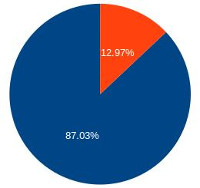
\includegraphics[width=0.22\textwidth]{./images/mdresult}}~~
\subfloat[Set of left mandibles.]{\label{figmgresult}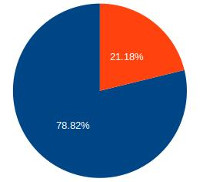
\includegraphics[width=0.22\textwidth]{./images/mgresult}}
\caption{The mean proportion of well and bad landmark locations of the two sets of left and right mandibles.}
\label{fig6}
\end{figure}

Beside the global results, we are also interested by the accuracy of
each estimated landmark. The error measure is the same with the first
one (distance between manual and corresponding estimated landmark) but
the acceptance is done with standard deviation of the distances
\cite{bland1996statistics}. Figs \ref{fig7} and \ref{fig8} show the
proportion of well estimated landmarks on each dataset. With 18
landmarks of right mandible, the highest proportion is belong to the
$1^{st}$ landmark with \textbf{98.62\%}; the lowest proportion is
\textbf{74.48\%} for the $14^{th}$ landmark. The remaining landmarks
are also estimated with a high accuracy greater than
\textbf{75\%}. For left mandibles, the highest and lowest success rate
are \textbf{93.01\%} for the $1^{st}$ landmark and \textbf{60.14\%}
for the $16^{th}$ landmark. In this evaluation, we can see that the
correct proportion on the $11^{th}$ and $12^{th}$ landmark of the left
mandible and the $13^{th}$ and $14^{th}$ landmark of the right
mandible are less than other landmarks. The reason is come from the
noise of the contours at the base of mandible is higher than the top
of the mandible. Currently, using SIFT to estimate the landmarks is
implemented in MAELab. It was written in C++. MAELab is distributed as
free library on the Github.

\begin{figure}[htb]
    \centering
    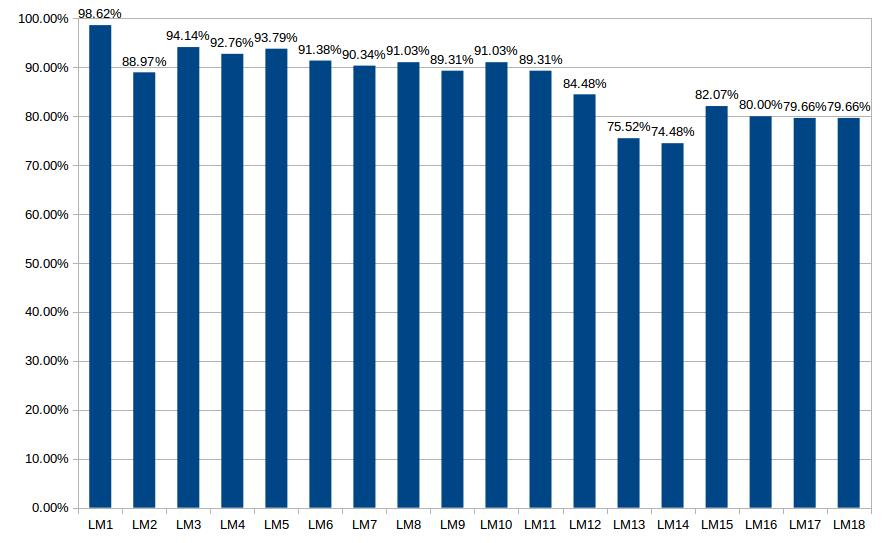
\includegraphics[width=0.5\textwidth]{./images/md_chartlms}
    \caption{The proportions of well estimated landmark for each model landmark of right mandibles.}
    \label{fig7}
\end{figure}
\begin{figure}[htb]
    \centering
    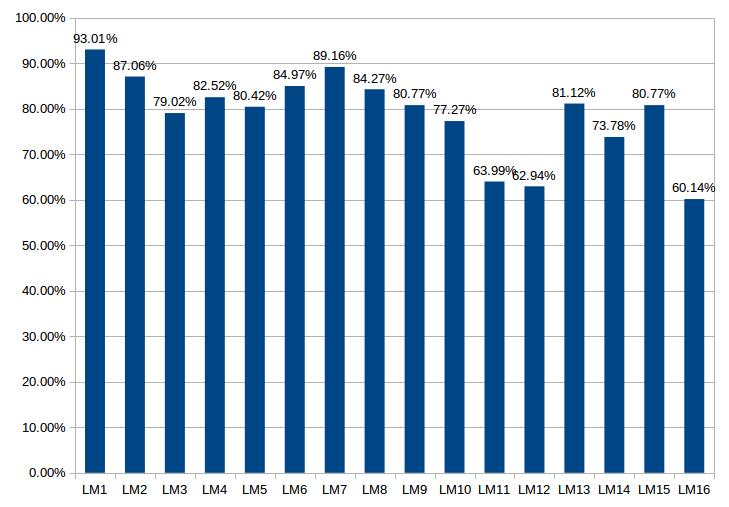
\includegraphics[width=0.5\textwidth]{./images/mg_chartlms}
    \caption{The proportions of well estimated landmark for each model landmark of left mandibles.}
    \label{fig8}
\end{figure}
\section{Conclusion and discussion}
The landmarks setting is the main way to analysis image in biology. In
this paper, we have described a difference way to use the SIFT
descriptor along with the segmentation and registration processes to
estimate the landmark on the beetle. Firstly, each mandible has been
segmented. Then, two contours are registered. Finally, SIFT descriptor
is applied to find the best matching position of estimated
landmarks. The results show that our method succeeds in locating all
the landmarks of the image. The accuracy of the method is sufficient
to be proposed to biologists as a replacement of the manual
measures. Moreover, considering with previous work
\cite{leestimating}, the position of the estimated landmarks are
improved a little bit. From now, the next stage consists the improving
to increase the correct accuracy of the landmarks in the bottom of the
mandible.


\bibliographystyle{plain}
\bibliography{references}

\end{document}
